


\begin{table}
{\scriptsize
\begin{center}
\begin{tabular}{|c||c|c|c|c|c||c|c|c|c|c|}
\hline
\hline
& \multicolumn{3}{|c|}{Program Source} & \multicolumn{1}{|c|}{Test Suite} \\
\hline
Subject & \#Classes. & \#Methods & SLOC & \#Test cases \\
\hline
\hline
{\tt Apache Commons} & & & & \\
{\tt Validator} & 64 & 578 & 6,033 & 434 \\
\hline
{\tt JExel 1.0.0} & & & & \\
{\tt beta 13} & 43 & 133 & 1,522	 & 344  \\
\hline
{\tt JAxen} & 167 & 1,078 & 12,462 & 2,138\\
\hline
{\tt JParser} & 115 & 178 & 3,046 & 647 \\
\hline
{\tt Apache Commons} & & & & \\
{\tt CLI} & 23 & 208 & 2,667 & 364 \\ 
\hline
\hline
\end{tabular}
\end{center}
}
\caption{Open Source Subject Programs}
\label{tab:opensourcesubs}
\end{table}



The SIR results show that reduction is useful for localization in an
idealized setting where suites are relatively complete and faults are
chosen for certain properties, and the Spidermonkey results show its
value in a particularly challenging setting (where passing tests have
very wide-ranging coverage).  How does reduction affect localization
in a typical open source project?

We attempted to answer this question by picking five open source Java
programs (shown in Table \ref{tab:opensourcesubs}) and a set of
identified and fixed bugs for those projects. We used patches that fixed the bugs to reproduce the bugs and then applied fault localization. Unfortunately, we found out that the dataset was not very helpful to effectively carry out fault localization.  In almost every case, only one test
case in the suite for the project caught the fault, and that test case
was, essentially, already minimal.  We examined a large number of bugs
in the bug repository for Validator and CLI and confirmed our
suspicion that this was very common: for most bugs, there was one,
near-minimal, test case.  The most test cases we saw for any bug was
four, and those were, again, near-minimal. Combining the project
suites and fixed bugs for these projects yielded a very uninteresting
localization problem, from our point of view.  Note that reduction was
not harmful or expensive, it simply \emph{made no real difference} for
this data set.  Why?

\subsubsection{The Bugs Researchers Don't See}

The following describes what we believe to be a common approach to
building up the test suite and bug database for a project:

\begin{enumerate}
\item Initially, a small set of tests are written to check for basic functionality of the system.
\item Before checking in new code, developers run the established
suite to make sure the code is largely correct.  The developer may add
tests for new functionality.
\item When users report a bug via the bug database that is not
detected by the current suite, developers add a new test (or a small
set of tests) to catch \emph{that fault}.  The fix for the bug is
often checked into the code repository at the same time.
\end{enumerate}


This is not an unreasonable approach, and roughly fits many
development models, including test-driven development.  The primary
deviations are that some projects don't maintain a good bug database
or add tests to catch all fixed bugs.  This workflow has two
unfortunate side effects for researchers, however.  First, note that
for bugs with entries in the bug database or fixes in the repository
(the common source of faults to use in evaluating localization or
testing methods), the test case(s) for the fault are likely to be
already near-minimal, because \emph{they are written specifically to
catch that bug.}  Second, if an existing, non-near-minimal test
``accidentally'' catches a bug during development, that bug
\emph{likely never makes it into the source history or bug database,
because a developer will fix it before checking in the code}.  The
primary exception is when a test added to catch a newly discovered
fault reveals older code that is also incorrect, for an unrelated
reason.  We speculate that this is a rare occurrence.  Together, these
two related issues mean that researchers using source history and the
bug database to investigate fault detection or localization tend to
see only a subset of the faults that have ever been present in some
version of the software \cite{Dangerous}.  There is a ``dark matter''
of bugs encountered during development that were detected and fixed
before they made it into the source repository.  Moreover, we
speculate that these bugs may be likely to have much more reducible
test cases than those that are visible to researchers using
traditional software history mining techniques, since no test case was
written for each bug.

This is particularly problematic for evaluation of fault localization,
because the bugs in the history may often not be the faults where a
developer could have benefited most from spectrum-based localization.
In many cases, we believe, the failing test case is produced based on
user bug reports, and by the time a test case exists, the bug is often
localized --- the test case is in many cases derived from the fix, not
the other way around!  There are, of course, various localization
techniques based on field reports, but these operate on less
information than traditional spectrum-based localizations.  We believe
there \emph{are} faults where spectrum-based localization would be
helpful: the ones in the ``dark matter,'' detected by a conscientious
developer running the regression suite before a check-in.  Some of
these bugs are surely trivial to understand, but many others may
require a fairly lengthy debugging session.  The value of localization
in this case, however, may be somewhat different than the typical
case.  We expect that developers will often have a good idea what the
faulty code is in these cases: it is probably code that just changed.
However, in other cases the newly added code may only expose a fault
in unchanged code.  The consequences of faulty new code may also be
hard to understand.  In both of these cases, good localization could
theoretically speed this ``invisible'' debugging process that (we
speculate with some support in the literature \cite{Dangerous}) often
leaves no trace in the bug database, source repository, or even
regression suite (the only trace might be lengthened time before the
developer commits).  The size and quality of ``dark matter'' bugs
needs serious investigation, if fault localization research is to be
responsive to real developer needs.

\subsubsection{Mutant-Based Evaluation}

\begin{figure}[t]
  \centering
  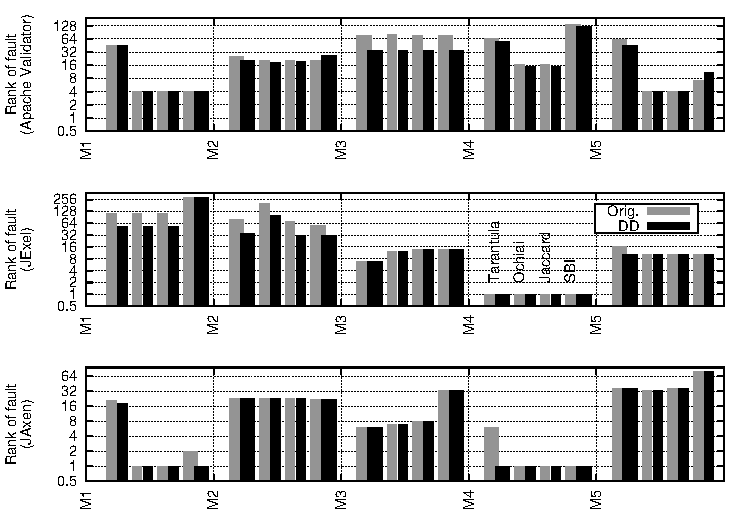
\includegraphics[width=\columnwidth]{opensource1}
  \caption{First Set of Open Source Results}
  \label{fig:opensource1}
\end{figure}

\begin{figure}[t]
  \centering
  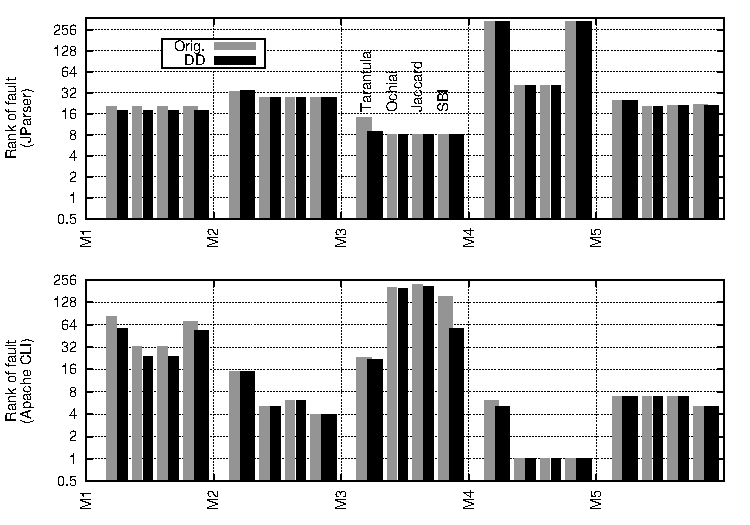
\includegraphics[width=\columnwidth]{opensource2}
  \caption{Second Set of Open Source Results}
  \label{fig:opensource2}
\end{figure}

There is no easy way to discover the missing bugs.  However, we want to evaluate how reduction can improve fault localization.  We therefore generated mutants for
each of the open source projects as it is being done in very recent fault localization literature to simulate bugs.[cite]  We do not claim that this
necessarily simulates small faults that might occur during development
but never make it into the test suite or bug database, only that it is
\emph{plausible} the small changes in mutants resemble invisible bugs.  A
mutant \cite{Mut2000} is a copy of the program with a single change to
its source code; mutants are often used to substitute for real faults
\cite{mutant}, including in recent fault localization work \cite{PureTest}.
Our strategy was to create mutants in the same way as Xuan and
Monperrus \cite{PureTest} in their own localization work, using 6
mutant operators.  From each set of mutants generated, we selected 5
or 6 mutants at random that met the following criteria: (1) the mutant
was killed by at least one test case and (2) the mutant generated no
errors in JUnit test cases.  A JUnit failure is caused by an
unsatisfied assertion, but an error is caused by another kind of test
failure, which may include some test setup or oracle problems.  Using
assertion failures only assures that we were remaining within the
intent of the original tests.

Figures \ref{fig:opensource1} and \ref{fig:opensource2} show the
results of applying reduction to these simulated faults.  Taking all
the open source projects and mutants together, we note that reduction
improved fault ranking in 51 cases, left it unchanged in 55 cases, and
made it worse in 2 cases.  The average improvement was 17.62 ranking
positions; the average negative effect size was 2 ranking positions.
The best improvement was 100
rank positions.  The average fault ranking without
reduction was 37.64 and with reduction it improved to 29.36.  However,
compared to switching from worst to best formula, reduction did not
perform as well here as with SIR or SpiderMonkey bugs: it was
 better to switch from worst to best formula in 14
cases, better to use reduction in 5 cases, and the methods were tied
in 8 cases.  Still, a simple, easily applicable method that is
sometimes better than \emph{knowing in advance which formula to use}
and almost never harmful (while switching formula is quite often
harmful, as the benefits of switching from worst to best formula show)
is a highly useful addition to fault localization practice.
